% ==================== 2 晶体学基础 ====================
\section{晶体学基础}

本章简要归纳晶体学的基础知识，说明如何描述晶体，为后续利用 Diamond 软件建立晶体结构
模型作准备。本章的主要内容与部分图例引自中央民族大学施洪龙老师的《X 射线晶体学》课程
课件\cite{shi2026xray}。

\subsection{晶体的基本性质}

晶体（crystal）是内部原子（或离子、分子）在三维空间呈周期性排列的固体。晶体具有以下
基本性质\cite{qin2004crystal}：

\begin{itemize}
  \item \textbf{长程有序性}：晶体内部的原子在很大范围内（纳米量级以上）保持周期性排列。
    长程有序是晶体区别于非晶体的本质特征，也是 X 射线衍射能够产生锐利衍射峰的根本原因。
  \item \textbf{均匀性}：晶体内部各部分的宏观性质（如化学组成、密度等）相同。
  \item \textbf{各向异性}：晶体在不同方向上的物理性质不同。例如电导率、热膨胀系数、
    折射率与机械强度随方向而异，这是不同方向上原子排列周期不同所决定的。
  \item \textbf{对称性}：晶体的外形及其物理、化学性质表现出特定的对称规律，这是晶体内
    原子周期排列的必然结果。
  \item \textbf{自范性}：晶体在生长过程中自发形成规则的多面体外形。晶面数 $F$、顶点数
    $V$ 与晶棱数 $E$ 之间满足欧拉定律 $F+V=E+2$。
  \item \textbf{具有确定的熔点}：同一结构晶体的键合方式相同，熔化断键所需能量相同，
    因此具有确定的熔点。
\end{itemize}

\begin{figure}[H]
  \centering
  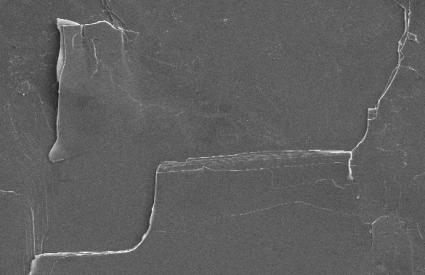
\includegraphics[width=0.42\textwidth]{assets/course/crystal-form.jpg}
  \caption{自发形成规则多面体外形的矿物晶体（引自施洪龙课件）}
  \label{fig:crystal-form}
\end{figure}

\subsection{晶体的描述}

描述晶体结构的基本要素包括：空间群（对称性）、晶格常数（晶胞形状）、原子类型、原子
坐标、占有率与位移因子（原子内容）。任何晶体结构都可表述为
\[
\text{晶体结构} = \text{点阵} + \text{结构基元}
\]
其中点阵是对晶体三维周期结构的数学抽象，基元是每个阵点所对应的原子（离子、分子）组。

\subsubsection{原胞与晶胞}

\textbf{点阵（lattice）}：将晶体中周期性重复的环境抽象为几何点（阵点），阵点在三维空间
按一定规律排列形成的无限阵列即为点阵。点阵的平移矢量为
\begin{equation}
  \bm{R}=h\bm{a}+k\bm{b}+l\bm{c} \qquad (h,k,l \text{ 为整数})
\end{equation}
式中 $\bm{a}$、$\bm{b}$、$\bm{c}$ 为基矢。晶体学中常用六种格子：初基 P、体心 I、面心 F、
底心 C、侧心 A、侧心 B（另有三方晶系的 R）。

\begin{figure}[H]
  \centering
  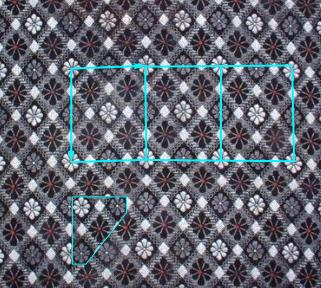
\includegraphics[width=0.4\textwidth]{assets/course/lattice-basis.jpg}
  \caption{点阵示意图：阵点与其平移矢量（引自施洪龙课件）}
  \label{fig:lattice-basis}
\end{figure}

\textbf{初基原胞（primitive cell）}：由三个不共面的基矢所围成的最小平行六面体重复单元。
初基原胞具有体积最小、只含一个格点的特点；但原胞取法不唯一，且往往不能反映晶体的对称性。
在密度泛函（如 VASP）等第一性原理计算中，使用原胞可减小计算量。

\begin{figure}[H]
  \centering
  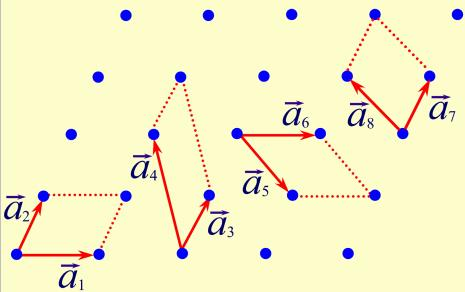
\includegraphics[width=0.5\textwidth]{assets/course/primitive-cell.jpg}
  \caption{由三个基矢构成的初基原胞（引自施洪龙课件）}
  \label{fig:primitive-cell}
\end{figure}

\textbf{晶胞（unit cell，结晶学原胞）}：能够完整反映晶体内部原子（离子）在三维空间分布
的化学--结构特征、并保持晶体对称性且体积尽量小的平行六面体。晶胞的形状由六个晶格参数
（晶格常数）$a$、$b$、$c$、$\alpha$、$\beta$、$\gamma$ 描述，其中 $\alpha=\angle(\bm{b},\bm{c})$、
$\beta=\angle(\bm{a},\bm{c})$、$\gamma=\angle(\bm{a},\bm{b})$。晶胞的选取遵循三条原则：
平行六面体中等棱等角的数目最多、直角最多、体积最小。

\begin{figure}[H]
  \centering
  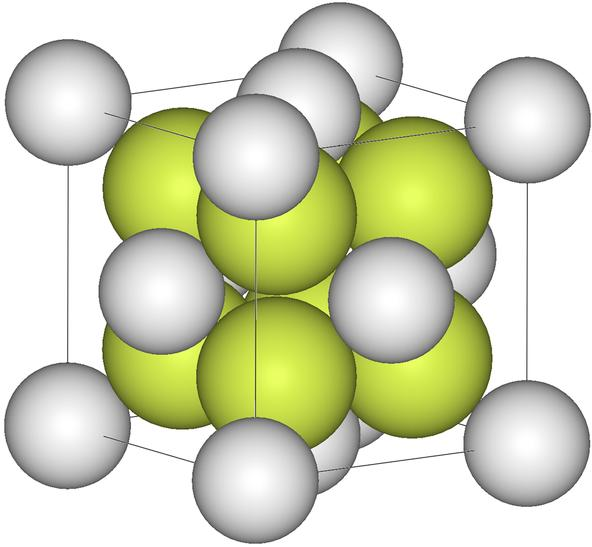
\includegraphics[width=0.45\textwidth]{assets/course/unit-cell.jpg}
  \caption{晶胞及其六个晶格常数 $a$、$b$、$c$、$\alpha$、$\beta$、$\gamma$
    （引自施洪龙课件）}
  \label{fig:unit-cell}
\end{figure}

晶胞与原胞之间可通过格点数建立联系。例如体心立方晶胞含 2 个格点，其初基原胞体积为晶胞
体积的 $1/2$，原胞基矢为
\begin{equation}
  \bm{a}_1=\tfrac{1}{2}(-\bm{a}+\bm{b}+\bm{c}),\quad
  \bm{a}_2=\tfrac{1}{2}(\bm{a}-\bm{b}+\bm{c}),\quad
  \bm{a}_3=\tfrac{1}{2}(\bm{a}+\bm{b}-\bm{c})
\end{equation}
面心立方晶胞含 4 个格点，其初基原胞体积为晶胞体积的 $1/4$，原胞基矢为
\begin{equation}
  \bm{a}_1=\tfrac{1}{2}(\bm{a}+\bm{b}),\quad
  \bm{a}_2=\tfrac{1}{2}(\bm{a}+\bm{c}),\quad
  \bm{a}_3=\tfrac{1}{2}(\bm{b}+\bm{c})
\end{equation}

\begin{figure}[H]
  \centering
  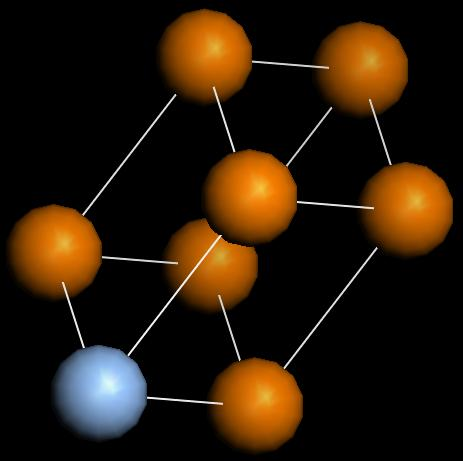
\includegraphics[width=0.4\textwidth]{assets/course/fcc-primitive.jpg}
  \caption{面心立方晶胞与初基原胞的结构模型（引自施洪龙课件）}
  \label{fig:fcc-primitive}
\end{figure}

图~\ref{fig:bcc-cell} 给出了体心立方晶胞与其初基原胞的关系：晶胞顶点与体心处各有一个
原子，虚线所示的初基原胞以晶胞顶点为顶点、以三个相邻晶胞的体心为其余顶点，只含一个格点。

\begin{figure}[H]
  \centering
  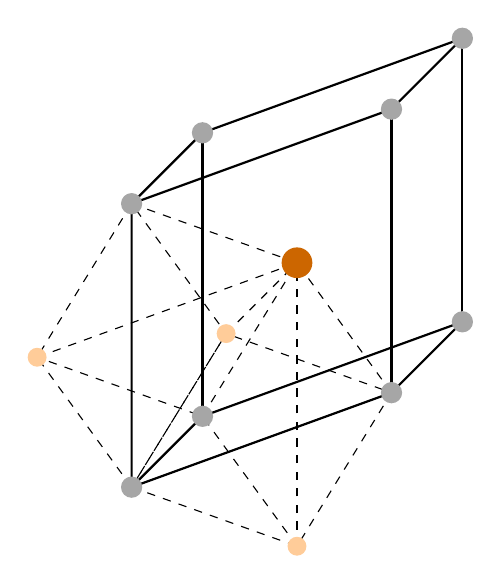
\begin{tikzpicture}[scale=1.5, line join=round]
    % 晶胞顶点（斜投影）：a=(2.2,0.8), b=(0.6,0.6), c=(0,2.4)
    \coordinate (O)   at (0,0);
    \coordinate (A)   at (2.2,0.8);
    \coordinate (B)   at (0.6,0.6);
    \coordinate (C)   at (0,2.4);
    \coordinate (AB)  at (2.8,1.4);
    \coordinate (AC)  at (2.2,3.2);
    \coordinate (BC)  at (0.6,3.0);
    \coordinate (ABC) at (2.8,3.8);
    % 体心
    \coordinate (cen) at (1.4,1.9);
    % 相邻晶胞体心（原胞其余顶点）
    \coordinate (P1) at (-0.8,1.1);  % 1/2(-a+b+c)
    \coordinate (P2) at (0.8,1.3);   % 1/2(a-b+c)
    \coordinate (P3) at (1.4,-0.5);  % 1/2(a+b-c)
    % 晶胞棱（实线）
    \draw[thick] (O)--(A)--(AB)--(B)--cycle;
    \draw[thick] (O)--(C)--(AC)--(ABC)--(BC)--(C);
    \draw[thick] (A)--(AC);
    \draw[thick] (B)--(BC);
    \draw[thick] (AB)--(ABC);
    % 原胞棱（虚线）
    \draw[dashed] (O)--(P1)--(C)--(P2)--cycle;
    \draw[dashed] (O)--(P3)--(A)--(P2);
    \draw[dashed] (O)--(P2);
    \draw[dashed] (P3)--(B)--(P1);
    \draw[dashed] (P3)--(cen);
    \draw[dashed] (P1)--(cen);
    \draw[dashed] (P2)--(cen);
    \draw[dashed] (A)--(cen);
    \draw[dashed] (B)--(cen);
    \draw[dashed] (C)--(cen);
    % 晶胞顶点原子
    \foreach \p in {O,A,B,C,AB,AC,BC,ABC} \fill[gray!70] (\p) circle (0.09);
    % 体心原子（较大）
    \fill[orange!80!black] (cen) circle (0.13);
    % 相邻晶胞体心（较小）
    \foreach \p in {P1,P2,P3} \fill[orange!40] (\p) circle (0.08);
  \end{tikzpicture}
  \caption{体心立方晶胞与初基原胞示意图。实线为晶胞，灰色球为晶胞顶点原子，深色球为
    体心原子；虚线平行六面体为初基原胞，其一个顶点在晶胞顶点处，其余三个顶点为相邻
    晶胞的体心原子（浅色球）。}
  \label{fig:bcc-cell}
\end{figure}

\subsubsection{对称性与空间群}

\textbf{宏观对称元素}指晶体的宏观性质所反映的对称性，包括四类独立对称元素：

\begin{itemize}
  \item \textbf{旋转轴 $n$}：晶体绕某一几何直线旋转 $2\pi/n$ 后复原。由于晶体周期性的
    限制，旋转轴只可能是 1、2、3、4、6 次轴。设沿周期方向相邻两阵点 A、B，绕 A 点轴
    旋转 $\theta$ 角后 B 移到 B$'$，B$'$ 仍必须是阵点，故
    $A'B'=AB-2AB\cos\theta=n\,AB$（$n$ 为整数），解得
    $\cos\theta = 0,\,\tfrac12,\,1$，对应 $\theta=90^\circ,60^\circ,0^\circ$（另一半解
    同理），即只存在 2、3、4、6 次轴。准晶（如 1984 年发现的五重对称准晶）因失去长程
    平移周期性而允许 5 次轴。
  \item \textbf{镜面 $m$}：晶体经某一平面反映后复原，操作前后两原子位于镜面同一法向的
    两侧且等距反向。
  \item \textbf{反演中心 $\bar{1}$}：晶体经某一点反演后复原，操作前后两原子位于同一直线
    上、等距反向。
  \item \textbf{旋转反演轴 $\bar{n}$}：旋转 $2\pi/n$ 与反演的联合操作。例如
    $\bar{3}=3+\bar{1}$，$\bar{6}=3/m$（三重旋转加镜面）。
\end{itemize}

\begin{figure}[H]
  \centering
  \subcaptionbox{(a) 旋转、反演与镜面操作示意}{%
    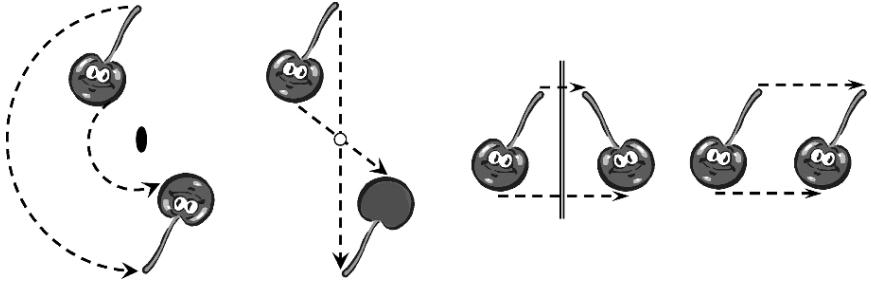
\includegraphics[width=0.62\textwidth]{assets/course/macro-sym.jpg}}

  \subcaptionbox{(b) 旋转轴次数的周期性证明示意}{%
    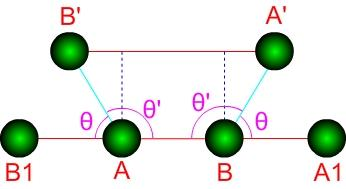
\includegraphics[width=0.55\textwidth]{assets/course/fivefold-proof.jpg}}
  \caption{宏观对称元素与晶体中旋转轴次数的限制（引自施洪龙课件）}
  \label{fig:macro-sym}
\end{figure}

\begin{figure}[H]
  \centering
  \subcaptionbox{(a) P1 与 P$\bar1$ 中反演中心的作用}{%
    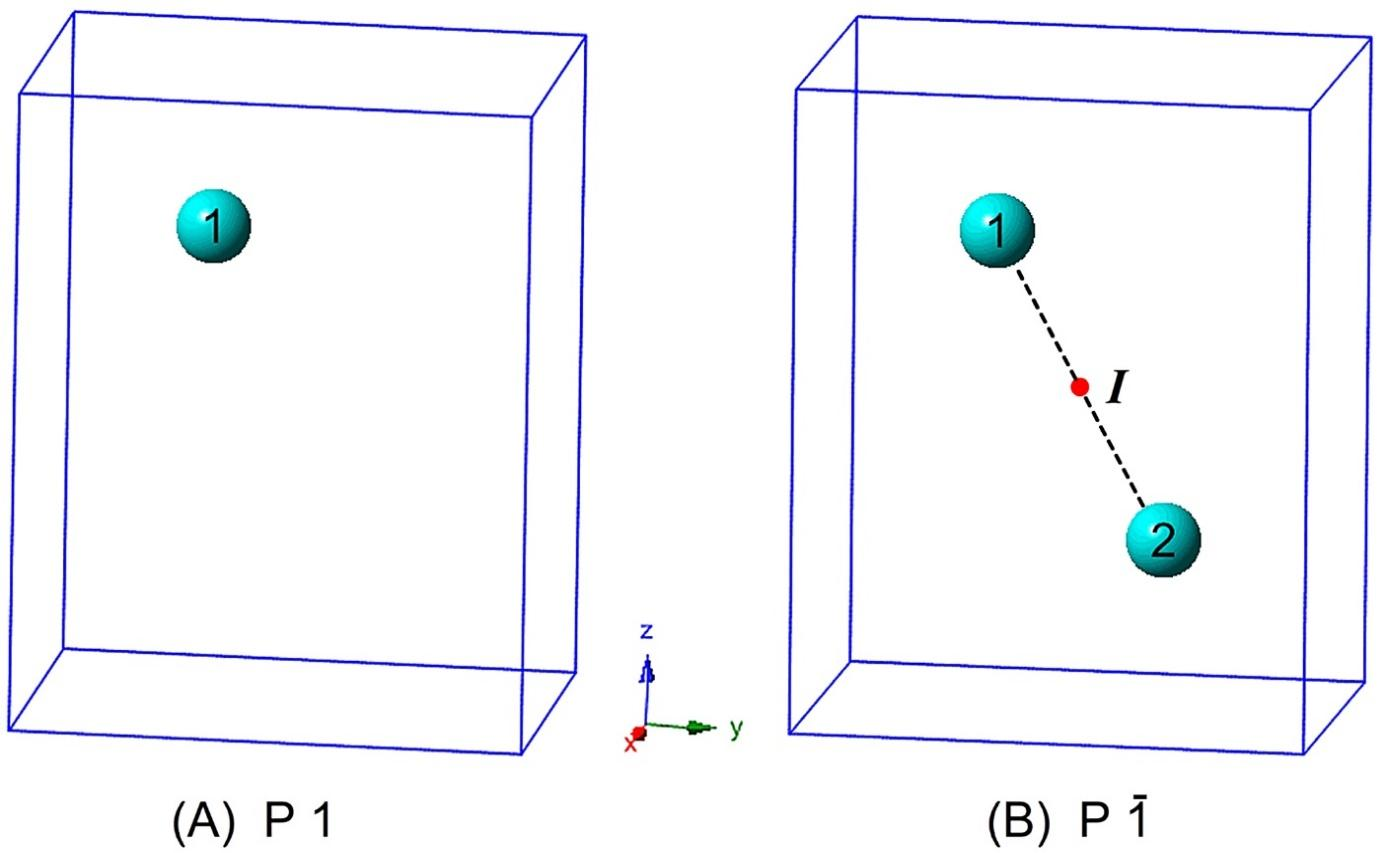
\includegraphics[width=0.52\textwidth]{assets/course/inversion.jpg}}

  \subcaptionbox{(b) P3、P$\bar3$、P6、P$\bar6$ 中的旋转轴与旋转反演轴}{%
    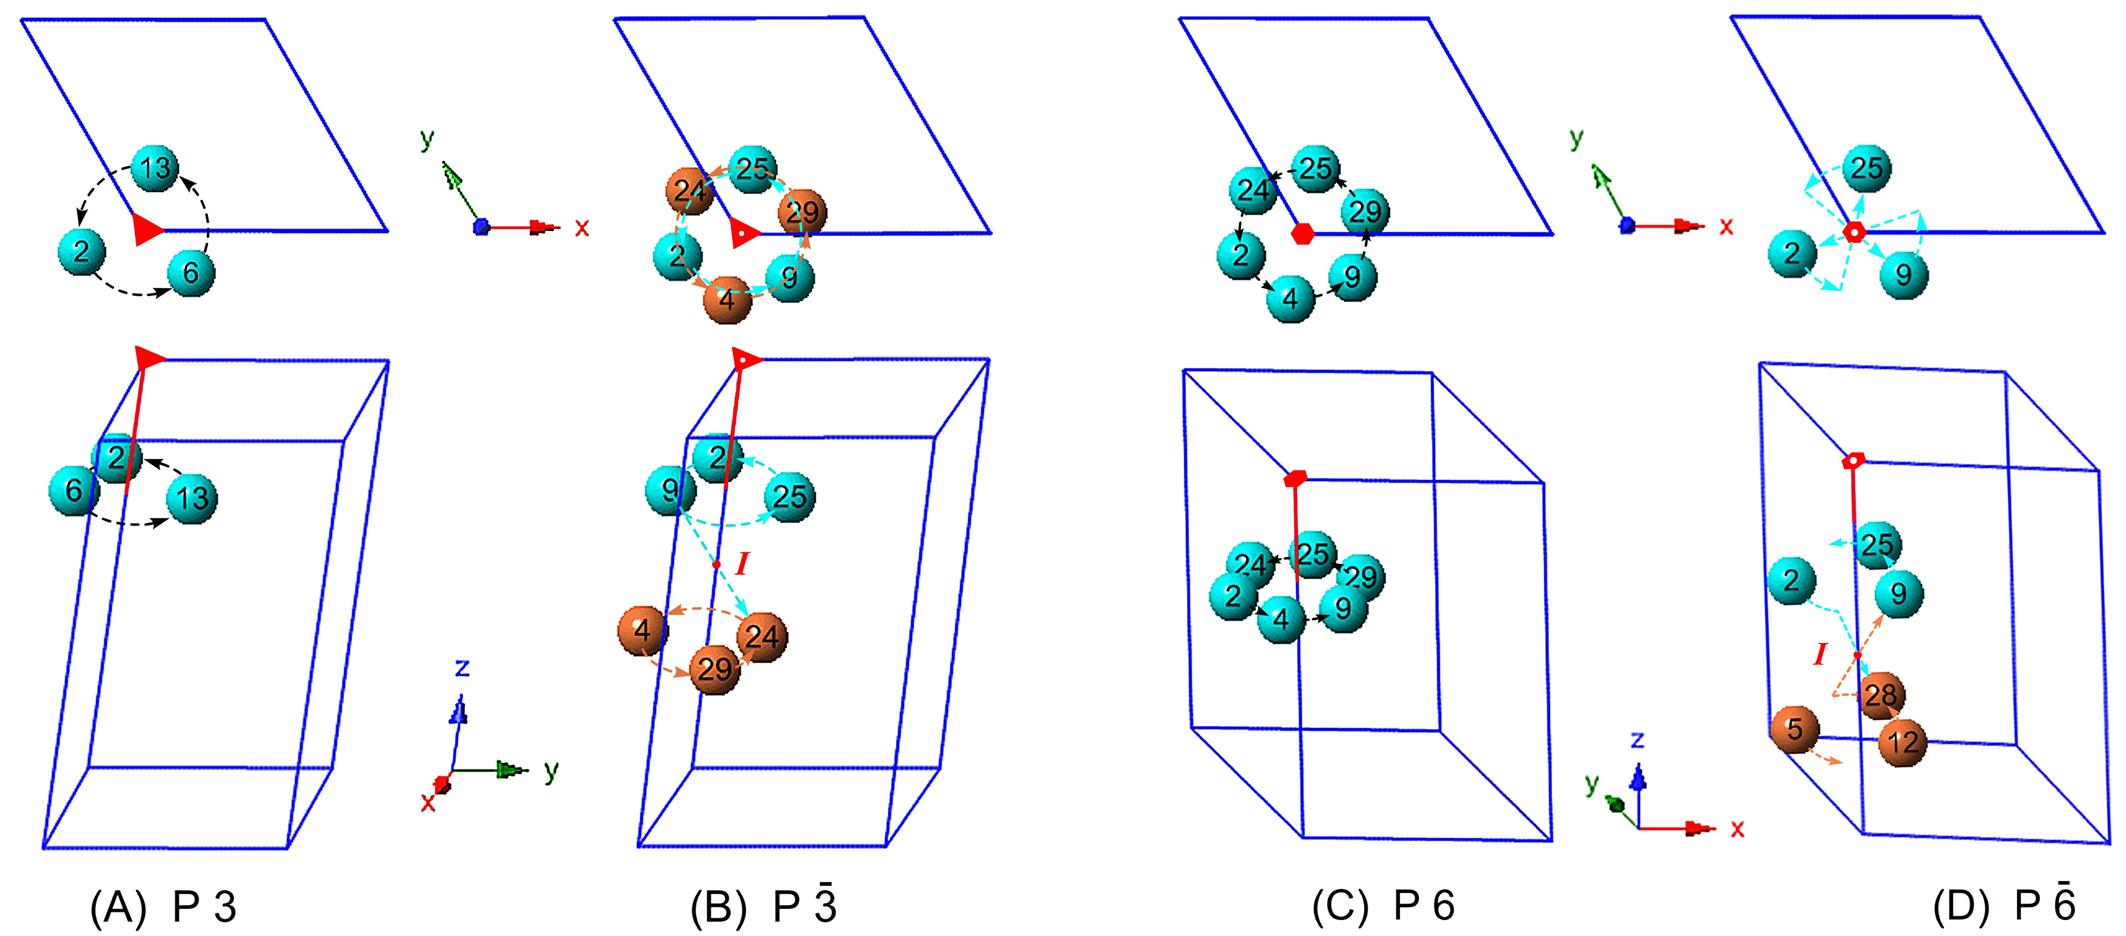
\includegraphics[width=0.5\textwidth]{assets/course/rotation-axis.jpg}}
  \hfill
  \subcaptionbox{(c) P$m$ 中的镜面操作}{%
    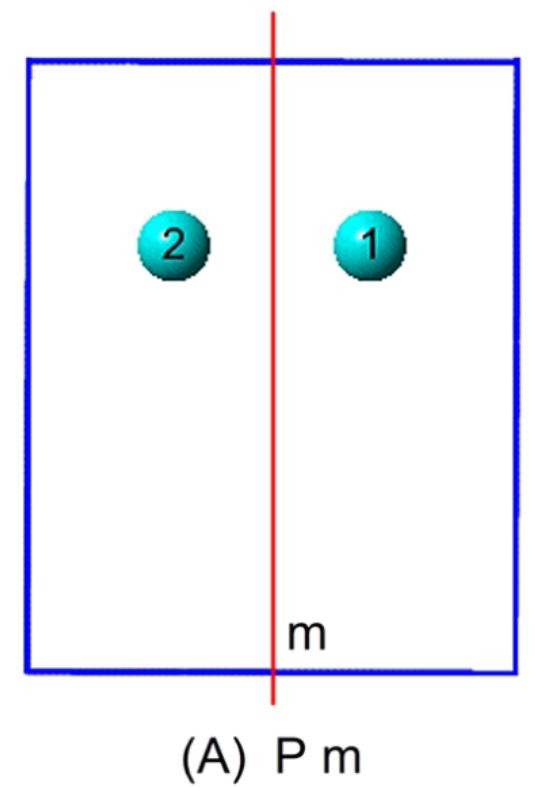
\includegraphics[width=0.24\textwidth]{assets/course/mirror.jpg}}
  \caption{利用 Diamond 观察宏观对称元素（引自施洪龙课件）}
  \label{fig:sym-diamond}
\end{figure}

宏观对称元素的组合共形成 \textbf{32 种点群}；按点群对称特征，晶体划分为 7 大晶系，
对应 14 种 Bravais 格子（表~\ref{tab:crystalsystems}）。在无限晶体中，平移本身也是
对称操作，并且还允许包含平移的\textbf{微观对称元素}——\textbf{螺旋轴}与\textbf{滑移
面}。螺旋轴 $n_m$ 是旋转 $2\pi/n$ 与沿轴方向平移 $m/n$ 个晶格周期单位的联合操作：经
$n$ 次操作后原子到达等效位置，而中间位置均不在同一平面上，沿轴呈螺旋状排列
（图~\ref{fig:micro-sym}(a)(b)）；滑移面是镜面反映与沿面内特定方向平移的联合操作，
包括沿 $a$、$b$、$c$ 方向平移 $1/2$ 的轴滑移面、沿面对角线方向平移 $1/2$ 的对角滑移面
$n$，以及平移 $1/4$ 的金刚石滑移面 $d$（图~\ref{fig:micro-sym}(c)）。宏观与微观对称
元素相互组合，共形成 \textbf{230 种空间群}\cite{hahn2005itt}。

\begin{figure}[H]
  \centering
  \subcaptionbox{(a) $6_1$ 螺旋轴的操作路径（旋转 $60^\circ$ 加平移 $1/6$）}{%
    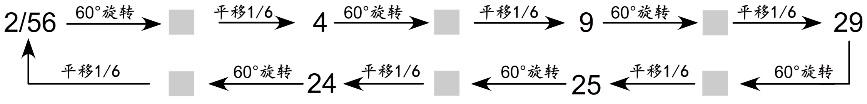
\includegraphics[width=0.82\textwidth]{assets/course/screw61.jpg}}

  \subcaptionbox{(b) $6_5$ 螺旋轴的操作路径（旋转 $300^\circ$ 加平移 $1/6$）}{%
    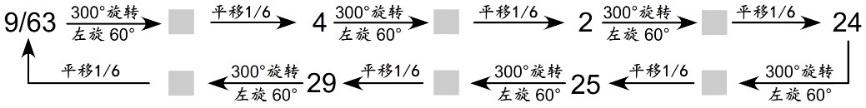
\includegraphics[width=0.82\textwidth]{assets/course/screw65.jpg}}

  \subcaptionbox{(c) $c$ 滑移面的操作（镜面加平移 $1/2$）}{%
    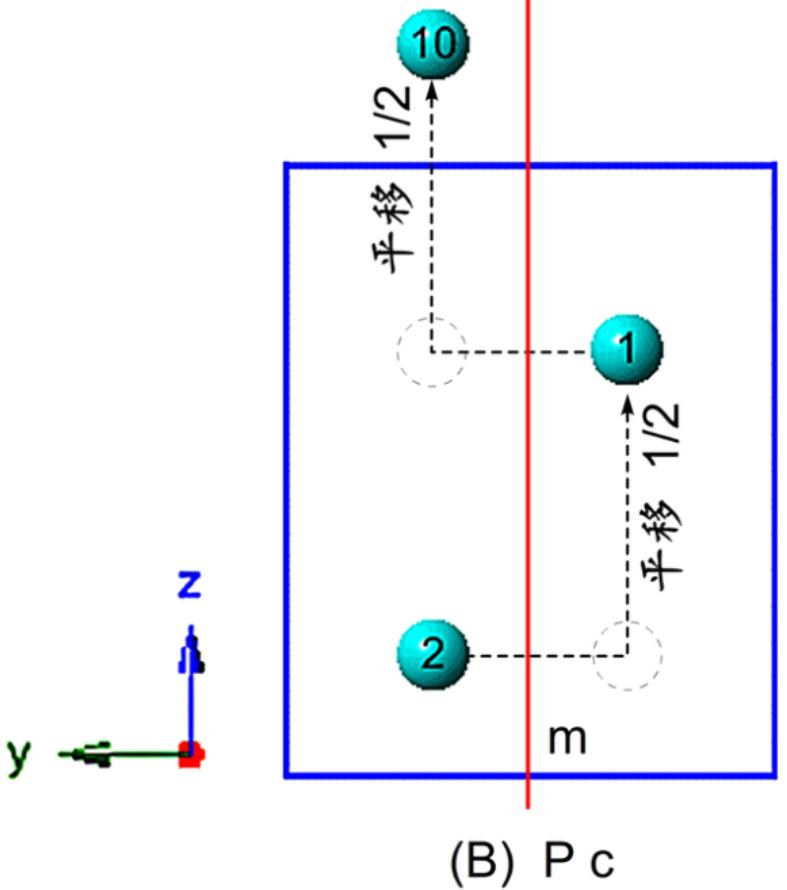
\includegraphics[width=0.3\textwidth]{assets/course/glide.jpg}}
  \caption{微观对称元素——螺旋轴与滑移面（引自施洪龙课件）}
  \label{fig:micro-sym}
\end{figure}

\begin{table}[H]
  \centering
  \small
  \caption{七大晶系、特征对称元素与 Bravais 格子}
  \label{tab:crystalsystems}
  \begin{tabular}{@{}llll@{}}
    \toprule
    晶系 & 晶格参数特征 & 特征对称元素 & Bravais 格子 \\
    \midrule
    三斜 & $a\ne b\ne c$，$\alpha\ne\beta\ne\gamma$ & 1 或 $\bar1$ & P \\
    单斜 & $a\ne b\ne c$，$\alpha=\gamma=90^\circ\ne\beta$ & 一个 2 次轴或镜面 & P, C \\
    正交 & $a\ne b\ne c$，$\alpha=\beta=\gamma=90^\circ$ & 三个互相垂直的 2 次轴（或镜面） & P, C, I, F \\
    四方 & $a=b\ne c$，$\alpha=\beta=\gamma=90^\circ$ & 一个 4 次轴 & P, I \\
    三方 & $a=b=c$，$\alpha=\beta=\gamma\ne90^\circ$ & 一个 3 次轴 & R \\
    六方 & $a=b\ne c$，$\alpha=\beta=90^\circ$，$\gamma=120^\circ$ & 一个 6 次轴 & P \\
    立方 & $a=b=c$，$\alpha=\beta=\gamma=90^\circ$ & 四个 3 次轴（沿体对角线） & P, I, F \\
    \bottomrule
  \end{tabular}
\end{table}

\begin{figure}[H]
  \centering
  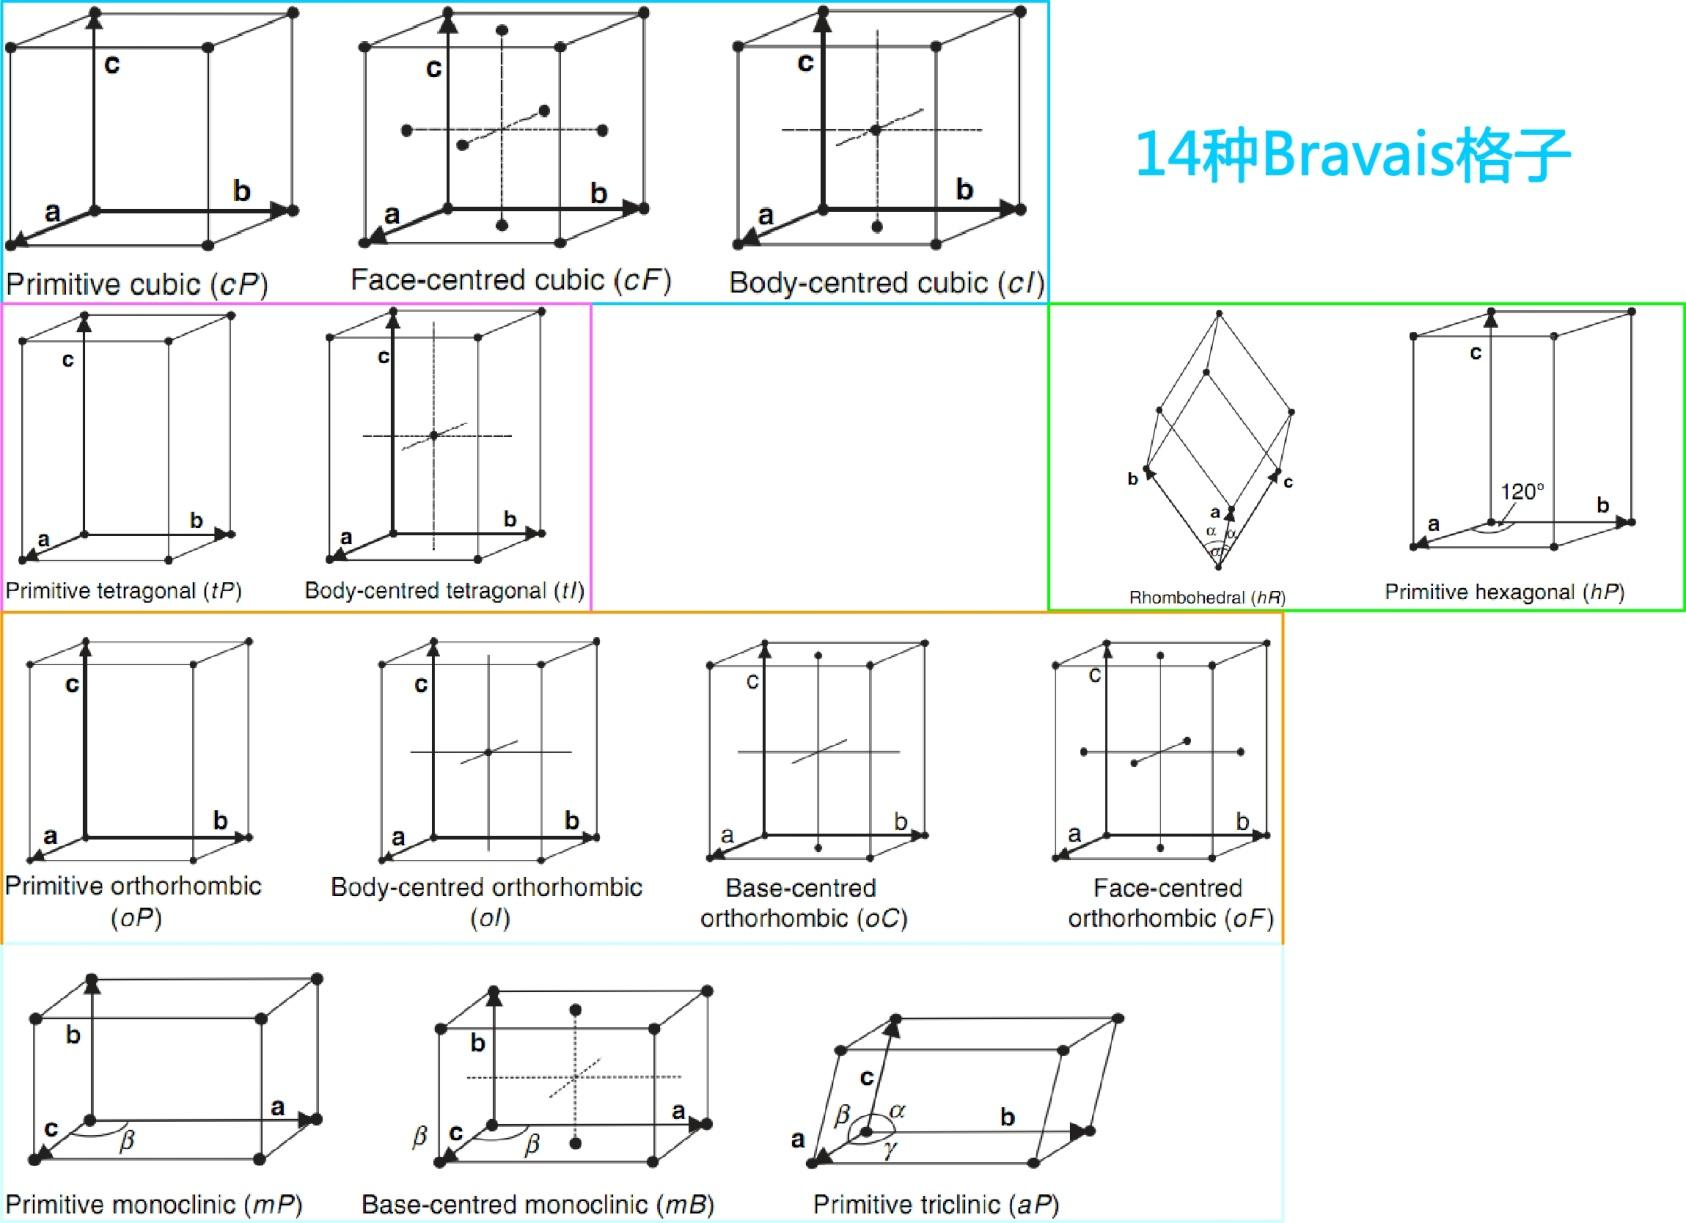
\includegraphics[width=0.75\textwidth]{assets/course/bravais-types.jpg}
  \caption{14 种 Bravais 格子（引自施洪龙课件）}
  \label{fig:bravais14}
\end{figure}

空间群的\textbf{国际符号}由点阵类型字母（P、F、I、A、B、C、R）与三个特征方向（由晶系
决定，见表~\ref{tab:crystalsystems}）上的对称元素符号组成。例如立方晶系的三个特征方向
依次为 [100]、[111]、[110]。据此：
$F\,m\,\bar3\,m$ 表示面心立方点阵，[100] 方向为镜面 $m$，[111] 方向为旋转反演轴
$\bar3$（立方晶系的特征），[110] 方向为镜面 $m$；$P\,6_3/m\,m\,c$ 表示六方初基点阵，
[001] 方向为 $6_3$ 螺旋轴加镜面，[100] 方向为镜面，[120] 方向为 $c$ 滑移面；
$P\,4_2/m\,n\,m$ 表示四方初基点阵，[001] 方向为 $4_2$ 螺旋轴加镜面；$I\,4_1/a\,m\,d$
表示体心四方点阵，[001] 方向为 $4_1$ 螺旋轴加 $a$ 滑移面，[100] 方向为镜面，[110]
方向为 $d$ 金刚石滑移面。

\begin{figure}[H]
  \centering
  \subcaptionbox{(a) 三斜至四方晶系}{%
    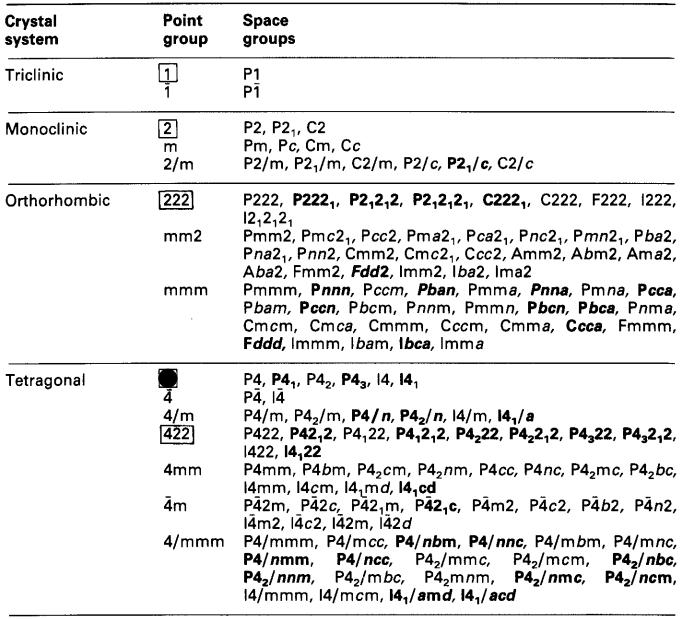
\includegraphics[width=0.42\textwidth]{assets/course/spacegroup-symbol.jpg}}
  \hfill
  \subcaptionbox{(b) 三方（六方）与立方晶系}{%
    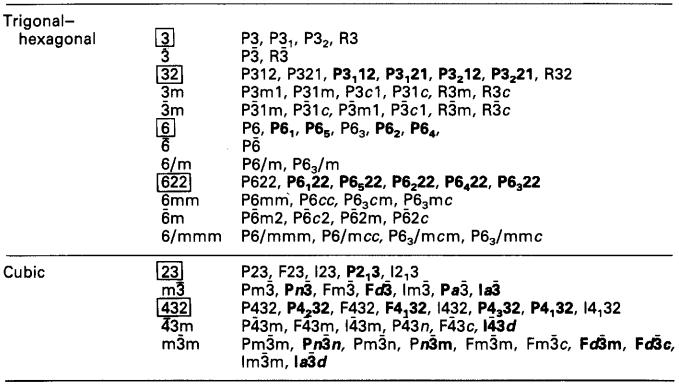
\includegraphics[width=0.42\textwidth]{assets/course/spacegroup-projection.jpg}}
  \caption{七大晶系中空间群与点群的对应关系（引自施洪龙课件）}
  \label{fig:spacegroup-table}
\end{figure}

\subsubsection{晶胞内的原子}

确定空间群与晶格常数后，还需给出晶胞内原子的\textbf{种类}、\textbf{分数坐标} $(x,y,z)$、
\textbf{占有率}（占位度）与\textbf{位移因子}（描述原子在平衡位置附近的热振动）等参数。
由于空间群对称操作的作用，只需给出非对称单元（asymmetric unit）中不等价原子的参数，
即可生成晶胞内全部等价原子。空间群表中以 \textbf{Wyckoff 位}给出各类可能占位：多重度
（multiplicity）表示在该位放一个原子时晶胞内出现几个等效原子，位点对称性（site
symmetry）表示该位所保持的对称性；多重度等于一般位置的多重度的位置称一般位，否则为
特殊位。

\begin{figure}[H]
  \centering
  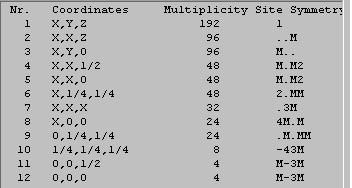
\includegraphics[width=0.6\textwidth]{assets/course/wyckoff-example.jpg}
  \caption{空间群表中的 Wyckoff 位表示例（引自施洪龙课件）}
  \label{fig:wyckoff}
\end{figure}

晶胞中的化学式单元数 $Z$ 可由实测密度与晶胞体积确定：
\begin{equation}
  Z=\frac{\rho V N_A}{M}
\end{equation}
其中 $\rho$ 为密度（g/cm$^3$）、$V$ 为晶胞体积（cm$^3$）、$N_A$ 为阿伏伽德罗常数、
$M$ 为摩尔质量。$Z$ 是检验指标化与结构解析结果是否合理的重要判据。将上述结构信息
（空间群、晶格参数与原子参数）按统一格式存储，即得到晶体学信息文件（CIF 文件），
它可被 Diamond 等软件直接读取用于建模。

\begin{figure}[H]
  \centering
  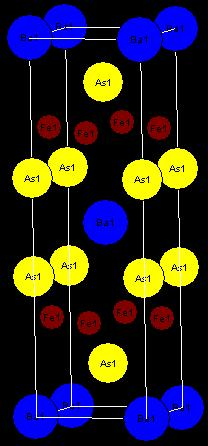
\includegraphics[width=0.28\textwidth]{assets/course/structure-elements.jpg}
  \caption{晶体结构模型示例：描述晶体结构所需的全部要素（空间群、晶格常数与原子参数）
    （引自施洪龙课件）}
  \label{fig:structure-elements}
\end{figure}
